\documentclass{article} % Tipo de documento

\usepackage[utf8]{inputenc} % Permite el uso de caracteres del Español

\usepackage[T1]{fontenc}

\usepackage{graphicx}

% Carátula del Artículo  

\title{Reporte de Actividad 4}

\author{Brenda Leyva Amaya}

\date{21 de febrero, 2018}
 
\begin{document}

\maketitle % Crea el título

\section{Introducción}

	En este documento incluimos la información relacionada a la cuarta práctica, en la cual tenemos un primer acercamiento a los archivos tipo script y algunos comandos para modificar y manipular dichos archivos. Los sistemas operativos tipo UNIX cuentan con un interprete de comandos llamado Shell, este actúa como un intermediario entre el usuario y el sistema operativo. Es como nos comunicamos con la computadora.
\vspace{0.5 cm}

Existen varios interpretes de tipo Shell, entre ellos están: C Shell (/bin/csh), Bourne Shell (/bin/sh), Korn Shell (/bin/ksh/), Bourne Again Shell (/bin/bash), y otros. Para Linux que es el sistema que utilizamos el "default" es /bin/bash. En esta actividades estaremos trabajando con Bourne Shell (/bin/sh) y Bourne Again Shell /bin/bash. 

\section{Generalidades de la Actividad.}

Como parte principal de esta actividad se trabajó con un script que descarga una serie de datos y los coloca en archivos para poder ser trabajados. A continuación practicamos con algunos comandos para observar lo que ellos generan. Los cuales se listan a continuación.

\vspace{0.5 cm}

\textbf{cat:}

\vspace{0.5 cm}

Este comando nos muestra los contenidos de un archivo y genera información a pantalla y cierra operación de manera inmediata, así se puede continuar dando instrucciones a terminal y en general interactuando con ella. La información que se generó permanece en la pantalla de la terminal. 

\vspace{0.5 cm}


\textbf{chmod:}

\vspace{0.5 cm}

Con este comando nos apoyamos para hacer modificaciones a los permisos de un documento/archivo así, decidimos quien puede verlo, modificarlo, o ninguna de las anteriores. 

\vspace{0.5 cm}


\textbf{echo:}

\vspace{0.5 cm}

Echo es el comando que imprime texto a terminal, este puede ser generado en la terminar misma o extraído de una página web o documento en especial.

\vspace{0.5 cm}


\textbf{grep:}  

\vspace{0.5 cm}

En ocasiones requerimos solo un cierto tipo de información contenida dentro de un archivo/documento, esta se puede filtrar con palabras clave que contienen o están relacionadas con dicha información y con la ayuda del comando "grep".

\vspace{0.5 cm}


\textbf{less:}  

\vspace{0.5 cm}

Less nos muestra la información contenida en un archivo y la despliega en pantalla continuando en dicho contenido como un comando que sigue trabajando hasta que nosotros decidamos cerrarlo, una vez cerrado la información desaparece de pantalla. 

\vspace{0.5 cm}


\textbf{ls:}

\vspace{0.5 cm}

Comando utilizado para conocer los contenidos dentro de una carpeta en específico, esto nos ayuda a confirmar la existencia de un documento o carpeta en el directorio en el cual nos encontramos trabajando.

\vspace{0.5 cm}


\textbf{wc:}

\vspace{0.5 cm}

"wc" es el comando "word count" como su nombre lo dice este nos permite obtener de manera rápida la cantidad de palabras que se encuentran contenidas en un archivo o en un segmento de archivo filtrado de manera específica de acuerdo a alguna característica o dato. 

\vspace{0.5 cm}


\textbf{Redirectores: |, >}  

\vspace{0.5 cm}
Utilizando los redirectores podremos crear cadenas de comando más complejas que contengan indicaciones muy específicas, estas se pueden utilizar con cada uno de los comandos que se han descrito en este documento. Por ejemplo no solo para conocer los contenidos de un archivo si no sólo una parte de este y además utilizando ">" podemos enviar este segmento o parte del archivo a un documento nuevo adicional. 


\section{Síntesis de notas de Steve Parker.}

Fuente: https://www.shellscript.sh/index.html
\vspace{0.5 cm}

El tutorial que se ha proporcionado en este sitio web tiene como propósito ayudar a entender algunos de los aspectos básicos de la programación en base a scripts en Shell. Bourne Shell fué escrito por Steve Bourne, así estos llevan su nombre, después se han escrito variadas versiones, este tutorial se enfoca principalmente en las versiones utilizadas en esta actividad. 
\vspace{0.5 cm}

Debido a un par de razones la programación de scripts en Shell no es bien vista por algunos programadores. Una de ellas es la velocidad a la cual correrá un programa en el interprete comparado con un programa en C, y que como se pueden hacer muy fácilmente estos scripts hay una gran cantidad de ellos de baja calidad. Un buen script deberá ser claro y evitar el uso de comandos innecesarios. 
\vspace{0.5 cm}

\subsection{Un primer script.}

Para un primer script se puede simplemente escribir una instrucción que escriba "Hello World" u "Hola mundo". Esto se puede llevar a cabo de la siguiente manera.

\begin{verbatim} 

#!/bin/sh
# This is a comment!
echo Hello World        # This is a comment, too!

\end{verbatim}

Echo se ha utilizado con un solo argumento, la liga "Hello world" e imprime esto exactamente. Ahora podemos jugar con el formato de impresión utilizando el siguiente script:

\begin{verbatim} 

#!/bin/sh
# This is a comment!
echo "Hello      World"       # This is a comment, too!
echo "Hello World"
echo "Hello * World"
echo Hello * World
echo Hello      World
echo "Hello" World
echo Hello "     " World
echo "Hello "*" World"
echo `hello` world
echo 'hello' world

\end{verbatim}

\subsection{Variables. Parte 1.}

Todo lenguaje de programación tiene el concepto de variables, esto es un nombre simbólico para un trozo de memoria al que se les asignarán valores para leerlos y manipularlos. El Bourne Shell no es excepción. Al definir variables no debe haber espacios entre el signo de igual, por ejemplo VAR=value. A continuación un ejemplo:

\begin{verbatim} 

#!/bin/sh
MY_MESSAGE="Hello World"
echo $MY_MESSAGE

\end{verbatim}

Shell no diferencia entre tipos de variables, no es necesario especificar el tipo, simplemente se declara la variable como tal. Sin embargo automáticamente identifica la naturaleza de dichas variables y sabe que no es posible operar por ejemplo la suma de una letra más un número.

\begin{verbatim} 

#!/bin/sh
x="hello"
expr $x + 1

expr: non-numeric argument

\end{verbatim}

Las variables en shell no requieren ser declaradas como en otros lenguajes, pero si se intenta leer una variable con caracteres que no se pueden reconocer el resultado es una linea vacía, no se tienen mensajes de error o advertencias. Esto puede causar algunos "bugs" sutiles. Por ejemplo:

Si se asigna: 
\begin{verbatim} 
MY_OBFUSCATED_VARIABLE=Hello
\end{verbatim}

y luego se llama de la siguiente manera:

\begin{verbatim} 
echo $MY_OSFUCATED_VARIABLE
\end{verbatim}

No se obtendrá nada ya que hubo un error al escribirla.

\subsection{Caracteres de Escape.}

La mayoría de los caracteres no son interpretados, es decir son tomados por shell literalmente si los ponemos entre comillas. Sin embargo algunos símbolos como: \begin{verbatim} ", $, `, y \ \end{verbatim} son interpretados por shell aún cuando estén indicados entre comillas 

\vspace{0.5 cm}

La diagonal es utilizada para marcar estos caracteres especiales para que no sean interpretados por shell y que pasen por el comando que se ha indicado. Se ha visto que las comillas son útiles para conservar espacios. El signo de dolar es especial porque marca una variable, la existencia de esta, la diagonal es especial pues se utiliza ella misma para marcar otros caracteres y dejarlos fuera, aquí un ejemplo de su uso:

\begin{verbatim} 

#!/bin/sh
echo "This is \\ a backslash"

# This is \ a backslash

echo "This is \" a quote and this is \\ a backslash"

# This is " a quote and this is \ a backslash

\end{verbatim}

Así que la diagonal misma debe ser indicada por si misma para poder ser mostrada no como parte del comando.

\subsection{Ciclos.}

La mayoría de los lenguajes tienen el concepto de ciclo (bucle o loop) Si se quiere repetir una tarea 20 veces, no es necesario generar el código 20 veces con quizá un pequeño cambio cada vez. Para esto se tienen "loops" en Bourne Shell. 

\vspace{0.5 cm}

Veamos un ejemplo de ciclo llamado "for" en shell: Generando la frase "Looping... number  " e indicando números del 1 al 5 en lugar de el espacio en blanco. 

\begin{verbatim} 

#!/bin/sh
for i in 1 2 3 4 5
do
  echo "Looping ... number $i"
done

\end{verbatim}

Veamos un ejemplo de ciclo llamado "while" en shell: Este script abrirá una interfaz que recupera todo aquello que se escriba y lo regresa a pantalla pero si se ingresa la palabra "bye" se sale del programa.

\begin{verbatim} 

#!/bin/sh
INPUT_STRING=hello
while [ "$INPUT_STRING" != "bye" ]
do
  echo "Please type something in (bye to quit)"
  read INPUT_STRING
  echo "You typed: $INPUT_STRING"
done

\end{verbatim}

Este es un ejemplo de ciclo con condición de salida flexible o dependiente del usuario.

\subsection{Test.}

Test se utiliza prácticamente por todos los scripts de shell, esto no es aparente pues no se le conoce como test en sí, se genera acceso simbólicamente con " [ ", y esto es para hacer los scripts más fáciles de leer.  Es también normalmente una función implícita de shell. Test es de hecho un programa como ls y otros, así que debe estar rodeado por espacios.

Su función principal es la comparación de valores, esto es de gran ayuda en tests lógicos. Como el ejemplo que sigue:

\begin{verbatim} 

#!/bin/sh
if  [ something ]; then
 echo "Something"
 elif [ something_else ]; then
   echo "Something else"
 else
   echo "None of the above"
fi

\end{verbatim}

Si se desea que los scripts trabajen  mejor, se deben revisar los contenidos de las variables antes de utilizar un test, algo como sigue:

\begin{verbatim} 

#!/bin/sh
echo -en "Please guess the magic number: "
read X
echo $X | grep "[^0-9]" > /dev/null 2>&1
if [ "$?" -eq "0" ]; then
  # If the grep found something other than 0-9
  # then it's not an integer.
  echo "Sorry, wanted a number"
else
  # The grep found only 0-9, so it's an integer. 
  # We can safely do a test on it.
  if [ "$X" -eq "7" ]; then
    echo "You entered the magic number!"
  fi
fi

\end{verbatim}

Esto es de gran utilidad para diseñar scripts más interactivos y flexibles.

\subsection{Case.}

La declaración "case" evita el atravesar una serie de relaciones "if .. then .. else" y es muy simple:

\begin{verbatim} 

#!/bin/sh

echo "Please talk to me ..."
while :
do
  read INPUT_STRING
  case $INPUT_STRING in
	hello)
		echo "Hello yourself!"
		;;
	bye)
		echo "See you again!"
		break
		;;
	*)
		echo "Sorry, I don't understand"
		;;
  esac
done
echo 
echo "That's all folks!"


\end{verbatim}

La linea "case" en sí siempre tiene el mismo formato y significa que estamos "testeando" el valor de la variable INPUT STRING. 

\subsection{Variables. Parte 2.}

Existe una serie de variables que están "listas para utilizarse" y la mayoría no pueden tener otros valores asignados a ellas. En estas puede haber información útil para el script acerca del ambiente en el cual está corriendo. Primero se revisarán las siguientes:

\begin{verbatim} 
 $0 .. $9 y $#
 \end{verbatim}

La primera es el nombre base del programa, como sea que este se haya guardado, las siguientes del 1 al 9 son los primeros 9 parámetros adicionales con que se llamó al script. La variable \$@ se refiere a todos los parámetros \$1, por otro lado \$* es similar pero no conserva el espacio ni comillas. Así la frase "File with spaces" se convierte en "File" "with" "spaces". Veamos un ejemplo de las mismas:

\begin{verbatim} 

#!/bin/sh
echo "I was called with $# parameters"
echo "My name is $0"
echo "My first parameter is $1"
echo "My second parameter is $2"
echo "All parameters are $@"

\end{verbatim}

Otra variable interesante es IFS, esta es el "Internal Field Separator" el separador interno de campos. Su valor predeterminado es SPACE TAB NEWLINE, pero si se va a cambiar es más fácil tomar una copia como se muestra en el siguiente ejemplo:

\begin{verbatim} 

#!/bin/sh
old_IFS="$IFS"
IFS=:
echo "Please input some data separated by colons ..."
read x y z
IFS=$old_IFS
echo "x is $x y is $y z is $z"

\end{verbatim}

\subsection{Variables. Parte 3.}

Al utilizar corchetes y el caracter especial ":-" se puede especificar un valor predeterminado para utilizarse si una variable no se ha armado o construido. 

\begin{verbatim} 

#!/bin/sh
echo -en "What is your name [ `whoami` ] "
read myname
echo "Your name is : ${myname:-`whoami`}"

\end{verbatim}

Esto se puede considerar un caso especial, se esta utilizando el comando whoami que envía a pantalla el nombre de login (UID). El ejemplo más canónico es aquel en que se utiliza texto fijo.

\begin{verbatim} 

#!/bin/sh
echo "Your name is : ${myname:-John Doe}"

\end{verbatim}

\subsection{Programas externos.}

Los programas externos son comúnmente utilizados con Shell, existen algunos comandos implícitos, pero muchos comandos utiles son de hecho utilidades de Unix como tr, grep, expr y cut. El acento inverso (`) está asociado a comandos externos y se utiliza para indicar texto "encerrado" que será ejecutado como comando. Veamos un ejemplo:

\begin{verbatim} 

#!/bin/sh
$ MYNAME=`grep "^${USER}:" /etc/passwd | cut -d: -f5`
$ echo $MYNAME
Steve Parker

\end{verbatim}

Vemos que este acento inverso simplemente toma la salida de un comando o serie de comandos que elegimos correr. También mejora el performance de algún comando o serie de comandos que tienden a ser lentos.

\begin{verbatim} 

#!/bin/sh
HTML_FILES=`find / -name "*.html" -print`
echo "$HTML_FILES" | grep "/index.html$"
echo "$HTML_FILES" | grep "/contents.html$"

\end{verbatim}

\subsection{Funciones.}

Una función en ocasiones ignorada de Bourne Shell en scripts es lo sencillo que es crear funciones para utilizarse dentro de un script. Esto se puede hacer de dos maneras, con un simple script en el cual la función se declara según el nombre dado el archivo en sí. Otra manera es crear una librería de funciones útiles y llamarlas al inicio de algún script. El enfoque será primeramente en la opción inicial. Una función podrá regresar un valor de una de cuatro maneras:

\vspace{0.5 cm}

Cambiando el estado de una variable o variables.

\vspace{0.5 cm}

Utilizando el comando de salida para finalizar el script en shell.

\vspace{0.5 cm}

Usando el comando de regreso para terminar la función y regresar a la sección normal del script.

\vspace{0.5 cm}

Una salida de echo a stdout, esto se tomaría por lo que la llama como c=`expr $a + $b`.

\vspace{0.5 cm}

Un simple script utilizando una función sería:

\begin{verbatim} 

#!/bin/sh
# A simple script with a function...

add_a_user()
{
  USER=$1
  PASSWORD=$2
  shift; shift;
  # Having shifted twice, the rest is now comments ...
  COMMENTS=$@
  echo "Adding user $USER ..."
  echo useradd -c "$COMMENTS" $USER
  echo passwd $USER $PASSWORD
  echo "Added user $USER ($COMMENTS) with pass $PASSWORD"
}

###
# Main body of script starts here
###
echo "Start of script..."
add_a_user bob letmein Bob Holness the presenter
add_a_user fred badpassword Fred Durst the singer
add_a_user bilko worsepassword Sgt. Bilko the role model
echo "End of script..."

\end{verbatim}

Una función se llamará en un "sub shell" si su salida se encuentra redirigida a algún otro lugar, esto es "myfunc 1 2 3 | tee out.log" seguirá diciendo "x is 1" en la segunda ocasión que se corra. Esto es porque un nuevo proceso de shell es llamado para redirigir myfunc(). Esto puede hacer que la actividad de "debugging" sea algo frustrante. Las funciones no pueden modificar los valores por los cuales han sido llamadas. Esto se debe hacer al cambiar las variables misma no los parámetros. Véase el siguiente ejemplo:

\begin{verbatim} 

#!/bin/sh

myfunc()
{
  echo "\$1 is $1"
  echo "\$2 is $2"
  # cannot change $1 - we'd have to say:
  # 1="Goodbye Cruel"
  # which is not a valid syntax. However, we can
  # change $a:
  a="Goodbye Cruel"
}

### Main script starts here 

a=Hello
b=World
myfunc $a $b
echo "a is $a"
echo "b is $b"

\end{verbatim}

\subsection{Pistas y consejos.}

En shell, grep es de gran utilidad para un programador, un ejemplo de esto sería:

\begin{verbatim} 

#!/bin/sh
steves=`grep -i steve /etc/passwd | cut -d: -f1`
echo "All users with the word \"steve\" in their passwd"
echo "Entries are: $steves"

\end{verbatim}

Otro comando común es tr, uno de sus usos es convertir texto de mayúsculas a minúsculas:

\begin{verbatim} 

#!/bin/sh
steves=`grep -i steve /etc/passwd | cut -d: -f1`
echo "All users with the word "steve" in their passwd"
echo "Entries are: "
echo "$steves" | tr ' ' '\012' | tr '[a-z]' '[A-Z]'

\end{verbatim}

Existen algunas cosas para las que shell no es muy bueno, dos herramientas muy útiles son sed y awk.

sed: Es un editor rápido de flujo, es capaz de buscar un patrón y aplicar transformaciones y/o comandos aún sencillos de combinar en filtros sofisticados pero sirviendo el propósito de modificar el texto en un flujo.

awk: La mayoría de las veces no es necesario combinar awk con otros filtros, su principal uso consiste en hacer modificaciones muy finas y modificaciones programáticas a un flujo de entrada.

\subsection{Referencias rápidas.}

Se incluye aquí una lista de comandos útiles que no es tan fácil memorizar:

\begin{center}
 	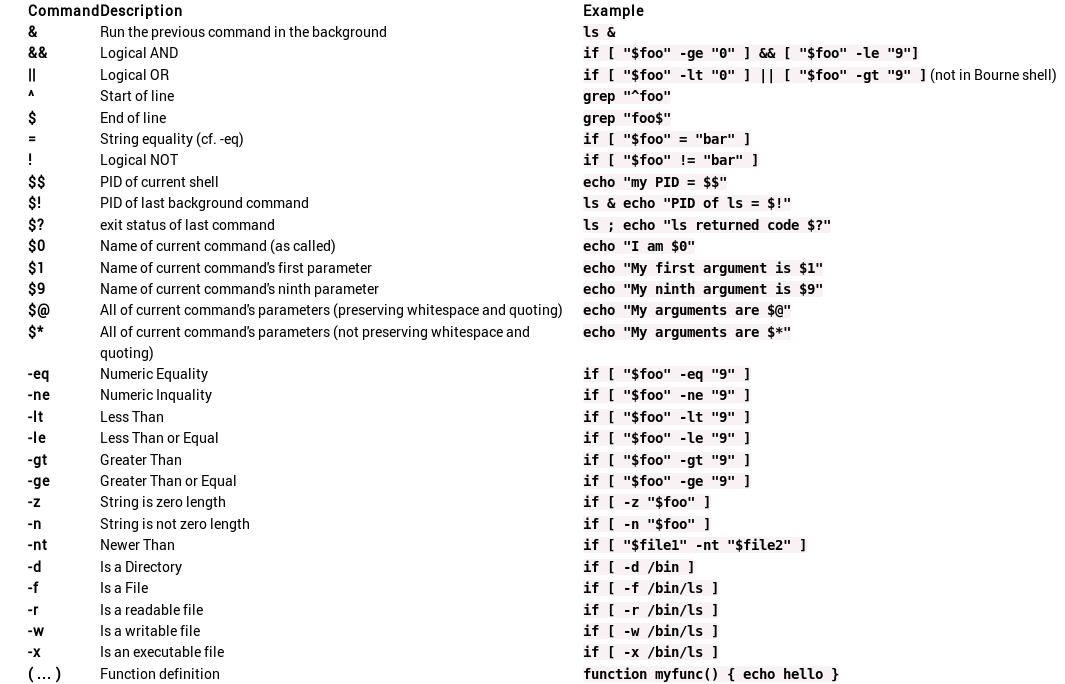
\includegraphics[width=15cm]{sheet.png}
 \end{center}

\subsection{Shell interactivo.}

En shell, bash tiene algunas herramientas muy útiles de búsqueda en historial, las flechas hacia arriba y hacia abajo navegaran a través del historial de comandos previos, mejor aún, la combinación Ctrl+r hará una búsqueda en reversa, haciendo comparación de cada parte de la linea del comando. Haciendo click en ESC y el comando seleccionado será seleccionado para el shell en uso para ser editado como sea requerido.

Por otro lado ksh se puede hacer mas útil al agregar comando del historial, si se desea comenzar una sesión en ksh desde otro shell interactivo simplemente se le llama de la siguiente manera:

\begin{verbatim} 

ksh$ # phew, that's better
ksh$ # do some stuff under ksh
ksh$ # then leave it back at the csh prompt:
ksh$ exit

\end{verbatim}


\section*{Apéndice:}

\hspace{0.45 cm} ¿Qué fue lo que más te llamó la atención en esta actividad?
\vspace{0.5 cm}

** Lo más interesante para mi fue el conocer los archivos tipo script como una nueva herramienta para desarrollar código y automatizar instrucciones. 

\vspace{0.5 cm}

¿Qué consideras que aprendiste?
\vspace{0.5 cm}

** Aprendí sobre la comunicación con el sistema operativo, vía comandos directamente vaciados en terminal así como aquellos colocados en un script que posteriormente se ejecuta.

\vspace{0.5 cm}

¿Cuáles fueron las cosas que más se te dificultaron?
\vspace{0.5 cm}

** El asimilar una cantidad mayor de información que en prácticas anteriores ya que se utilizaron muchas herramientas nuevas en esta ocasión.

\vspace{0.5 cm}

¿Cómo se podría mejorar en esta actividad?
\vspace{0.5 cm}

** Dando oportunidad de tomar nota sobre los comandos cuando se están poniendo en uso y cuando estos son indicados por el profesor ya que dichas notas hubiesen sido de enorme ayuda para la realización del presente reporte. Se podría decir que esto sería una pequeña porción de la clase dedicada a contenidos más teóricos.

\vspace{0.5 cm}

¿En general, cómo te sentiste al realizar en esta actividad? 
\vspace{0.5 cm}

** En esta ocasión el tiempo se sintió un poco menos suficiente que en las actividades anteriores por lo cual quizá se sacrificó un nivel de calidad por un producto entregado en el tiempo especificado. 

\vspace{0.5 cm}


 
\end{document}